\documentclass{../source/zjureport}

\major{信息工程}
\name{邓智城}
\title{实验设计报告}
\stuid{3190101704}
\college{信息与电子工程学院}
\grades{}
\date{2022年3月10日}
\lab{东4-319}
\course{通信原理实验}
\instructor{金向东、龚淑君}
\expname{小信号调谐放大器}
\exptype{综合}
\partner{王瑜昕}

\begin{document}
	\makecover
    \makeheader
    \section{实验目的和要求}
    (1)掌握小信号调谐放大器的工作原理。
    
    (2)掌握频谱分析仪的基本使用方法。
    
    (3)掌握调谐放大器电压增益、通频带及选择性的定义、测试及计算方法。

    \section{实验原理}
    小信号调谐放大器广泛用作高频和中频放大器,特别是用在通信接收端的前端电路,其主要目的就是实现对高频小信号的放大。
    
    小信号调谐放大器的幅频特性:
    \begin{figure}[H]
    	\centering
    	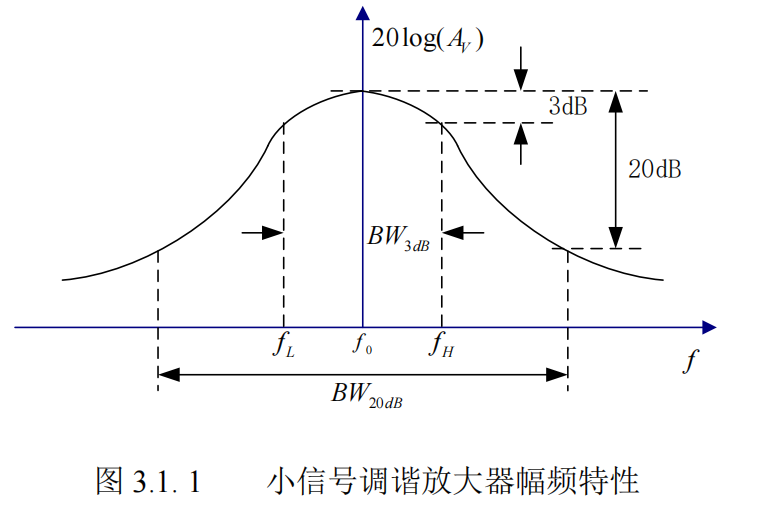
\includegraphics[scale=0.4]{figure/fig1.png}
    \end{figure}
    
    调谐放大器特性测试采用扫频法,采用带跟踪源的频谱仪进行测试。
    
    \section{实验电路分析}
    实验电路图:
    
    \begin{figure}[H]
    	\centering
    	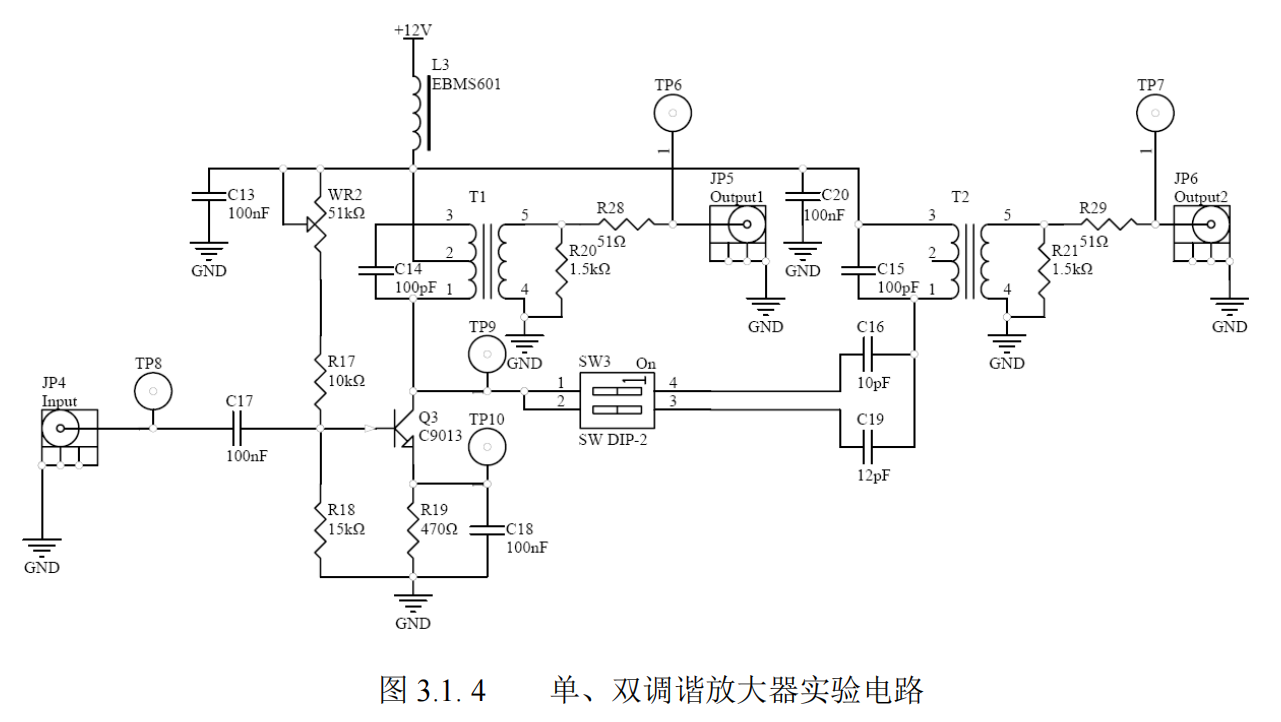
\includegraphics[scale=0.4]{figure/fig2.png}
    \end{figure}
	
	SW3为一个两位拨码开关,“0”为“OFF”,“1”为“ON”。当状态为“00”时,即没有接入任何耦合电容时,电路为单调谐放大器;状态为“01”“10”或“11”时,即电路接入任意不同电容时,电路为双调谐放大器。另接入JP5为单调谐放大器,接入JP6为双调谐放大器。
	电阻WR2为基极偏置电阻,R19为射极电阻,两者与电阻R17、R18共同决定晶体管的静态工作点。因而令WR2为可变电阻即可改变晶体管的静态工作点,从而来改变放大器的增益。
	
	\section{操作方法和实验步骤}
	\subsection{单调谐小信号放大器实验}
	(1)开关设置为“00”状态,频谱分析仪接入输出信号端信号JP5。调节静态工作点,使$V_{EQ} = 1.5V$,由$R_{19} = 470\Omega$得$I_{EQ} = 3.19 mA$。
	
	(2)设置频谱分析仪的参数如下:
	频谱分析仪中心频率为10.7MHz;扫宽度为20MHz;参考电平为20dBm;设定输出功率为-20dBm后打开跟踪源。即可获得小信号调谐放大器的传输特性曲线。
	
	
	(3)利用“peak”功能获得谐振频率。
	
	(4)通过谐振频率与输入功率可以获得功率增益。
	
	(5)利用“marker”功能获取3dB通频带,即$BW_{3dB}$。
	
	(6)同(5)获得20dB通频带,即$BW_{20dB}$。通过$BW_{20dB}$与$BW_{3dB}$的比值可以获得电路的选择性。
	
	(7)调节可变电阻WR2使得静态工作点改变,对比不同静态工作点下的调谐放大器的谐振增益和带宽。
	
	\subsection{双调谐小信号放大器实验}
    (1)将频谱分析仪从IP5端调节至JP6端。调节开关状态为“01”、“10”、“11”。观测三个条件下放大器的传输特性。
    
    (2)在开关未“01”状态下,测试谐振增益、通频带、矩形系数,并与单调谐放大器时进行比较。
	
	\section{实验数据整理和分析}
	\subsection{单调谐小信号放大器实验}
	\subsubsection{晶体管的静态工作点调整}
	晶体管的静态工作点 $I_{EQ} = 3.1915mA$
	\subsubsection{频谱分析仪设置}
	小信号调谐放大器的传输特性曲线忘了拍照。
	\subsubsection{谐振频率测试}
	谐振频率=$10.6666MHz$
	\subsubsection{谐振增益测试}
	$P_o = 3.30dBm,P_i=-20dBm,G=P_o-P_i = 23.30dBm$
	\subsubsection{通频带测试}
	3dB通频带:$BW_{3dB}=700kHz+800kHz=1500kHz$
	\subsubsection{选择性测试}
	20dB带宽:$BW_{20dB}=10.067MHz+4.53MHz=14.597MHz$
	
	矩形系数:$K_{v0,1}=\frac{BW_{20dB}}{BW_{3dB}}=\frac{14597}{1500}=9.73133$,说明选择性不是很理想。
	
	\subsubsection{静态工作点对谐振放大器增益的带宽的影响}
	在输入为-20dBm 不变的条件下,将晶体管的工作电流
	IC 从 1mA 调整到 5mA,测量其谐
	振增益和带宽结果如下:
	
	\begin{center}
		\begin{math}
			\begin{array}{|c|c|c|c|c|c|}
				\hline \text{工作电流}(mA) & 1 & 2 & 3 & 4 & 5 \\
				\hline \text{输出功率}(dBm) & -6.33& -0.44& 2.72& 4.86& 6.37\\
				\hline \text{谐振增益}(dB) &13.67&19.56 &22.72 &24.86 &26.37 \\
				\hline 3dB\text{带宽}(kHz) &1533.32&1533.33&1533.33&1566.66& 1600\\
				\hline
			\end{array}
		\end{math}
	\end{center}
	
	\begin{figure}[H]
		\centering
		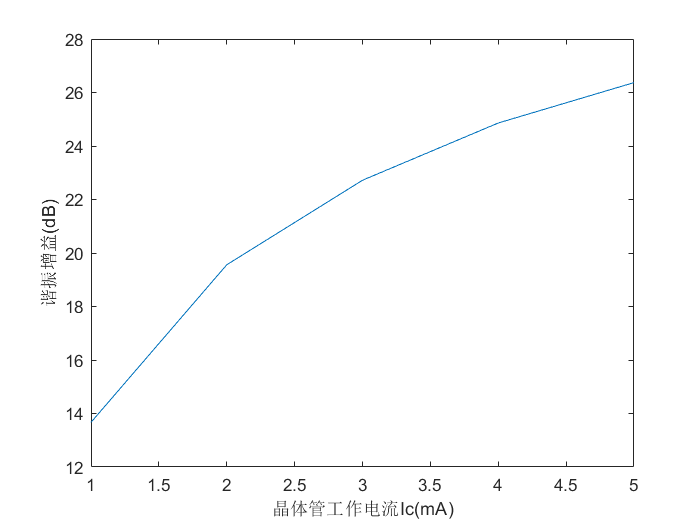
\includegraphics[scale=0.7]{figure/gain.png}
	\end{figure}
	从图中我们可以看出:随着工作电流的增加,谐振功率近似线性增加。
	
	而3dB带宽基本不变。
	
	\subsection{双调谐小信号放大器实验}
	\subsubsection{耦合状态观测}
	分别将 SW3 设成“10”、“01”
	和“11”,观测在弱耦合、临界耦合和强耦合条件下放大器的传输特性。
	
	(1)弱耦合状态:幅频特性为单峰
	\begin{figure}[H]
		\centering
		\includegraphics[width = 8cm]{figure/ruo.jpg}
		\caption{弱耦合状态下的放大器传输特性曲线}
	\end{figure}
	\newpage
	(2)临界耦合状态:幅频特性为双峰
	\begin{figure}[H]
		\centering
		\includegraphics[width = 8cm]{figure/linjie.jpg}
		\caption{临界耦合状态下的放大器传输特性曲线}
	\end{figure}
	(3)强耦合状态:双峰,顶部相对临界耦合偶尔而言更宽
	\begin{figure}[H]
		\centering
		\includegraphics[width = 8cm]{figure/qiang.jpg}
		\caption{强耦合状态下的放大器传输特性曲线}
	\end{figure}

	\subsubsection{谐振增益测试}
	在临界耦合状态下,双调谐放大器的谐振增益为23.08dBm。
	
	比单调谐放大器的谐振增益=23.30dBm略小。
	\subsubsection{通频带测试}
	在临界耦合状态下,双调谐放大器的3dB通频带为933.33kHz。
	
	比单调谐放大器的3dB通频带=1500kHz要小一些。
	\subsubsection{选择性测试}
	在临界耦合状态下,$BW_{20dB}=2.2MHz+1.1MHz=3.3MHz。$
	
	矩形系数$=\frac{3300}{933.33}=3.5357$,比单调谐放大器的矩形系数9.73要小很多,说明双调谐放大器滤除邻近波道干扰信号的能力比单调谐放大器更好。
	
	\section{思考题}
	\subsection{高频小信号放大器的主要技术指标有哪些?}
	
	谐振频率、谐振增益、通频带、增益带宽积、选择性、噪声系数
	
	\subsection{单级单调谐放大器的电压增益与那些因素有关?当谐振回路中的并联电阻R变化时,增益及带宽将怎样变化?当谐振放大器的静态工作点变化时,增益及带宽将怎样变化?}
	
	单级单调谐放大器的电压增益与三极管的正向传输导纳、负载导纳、谐振回路导纳、接入系数等有关,也与晶体管的电流放大系数、谐振电路的品质因数等有关。
	
	若R已使电路谐振,增大R值会使电压增益变大,带宽变小(增益带宽积基本不变)。
	随着静态工作电流变大,增益增加及带宽变化很小。

	\subsection{回路的谐振频率和那些参数有关?如何判断谐振回路处于谐振状态?}
	
	主要与L、C有关。当功率增益达到最大时即处于谐振状态。
	
\end{document}